\subsection*{Problema 02}

\textbf{Enunciado:} Calcular la integral:
\begin{equation*}
\int \dfrac{(x-1)dx}{3x^2 - 4x + 3}
\end{equation*}

\textbf{Solución:} 
Primero, analizamos el denominador 
$D(x) = 3x^2 - 4x + 3$. 
Su discriminante es $\Delta = (-4)^2 - 4(3)(3) = 16 - 36 = -20 < 0$, 
por lo que es irreducible en los reales. La derivada 
del denominador es $D'(x) = 6x - 4$.

Modificamos el numerador para que contenga 
a $6x - 4$:
\begin{align*}
x - 1 &= \dfrac{1}{6}(6x - 6) \\
&= \dfrac{1}{6}(6x - 4 - 2)
\end{align*}

Sustituimos esto en la integral original:
\begin{align*}
I &= \int \dfrac{\frac{1}{6}(6x - 4 - 2)}{3x^2 - 4x + 3} dx \\
&= \dfrac{1}{6} \int \dfrac{6x - 4}{3x^2 - 4x + 3} dx \\
&\quad - \dfrac{2}{6} \int \dfrac{dx}{3x^2 - 4x + 3}
\end{align*}

La primera integral es inmediata por sustitución 
$u = 3x^2 - 4x + 3$:
\begin{equation*}
I_1 = \dfrac{1}{6} \ln|3x^2 - 4x + 3|
\end{equation*}

Para la segunda integral, completamos cuadrados 
en el denominador:
\begin{align*}
3x^2 - 4x + 3 &= 3\left(x^2 - \dfrac{4}{3}x + 1\right) \\
&= 3\left[\left(x - \dfrac{2}{3}\right)^2 + \dfrac{5}{9}\right]
\end{align*}

Sustituimos esto en la segunda integral:
\begin{align*}
I_2 &= -\dfrac{1}{3} \int \dfrac{dx}{3\left[\left(x - \dfrac{2}{3}\right)^2 + \dfrac{5}{9}\right]} \\
&= -\dfrac{1}{9} \int \dfrac{dx}{\left(x - \dfrac{2}{3}\right)^2 + \left(\dfrac{\sqrt{5}}{3}\right)^2}
\end{align*}

Aplicando la fórmula de la arcotangente:
\begin{align*}
I_2 &= -\dfrac{1}{9} \left(\dfrac{3}{\sqrt{5}}\right) 
\arctan\left(\dfrac{x - \frac{2}{3}}{\frac{\sqrt{5}}{3}}\right) \\
&= -\dfrac{1}{3\sqrt{5}} \arctan\left(\dfrac{3x - 2}{\sqrt{5}}\right)
\end{align*}

Combinando ambos resultados, la solución general 
es:
\begin{align*}
I &= \dfrac{1}{6} \ln(3x^2 - 4x + 3) \\
&\quad - \dfrac{\sqrt{5}}{15} \arctan\left(\dfrac{3x - 2}{\sqrt{5}}\right) + C
\end{align*}

\begin{figure}[H]
	\centering
	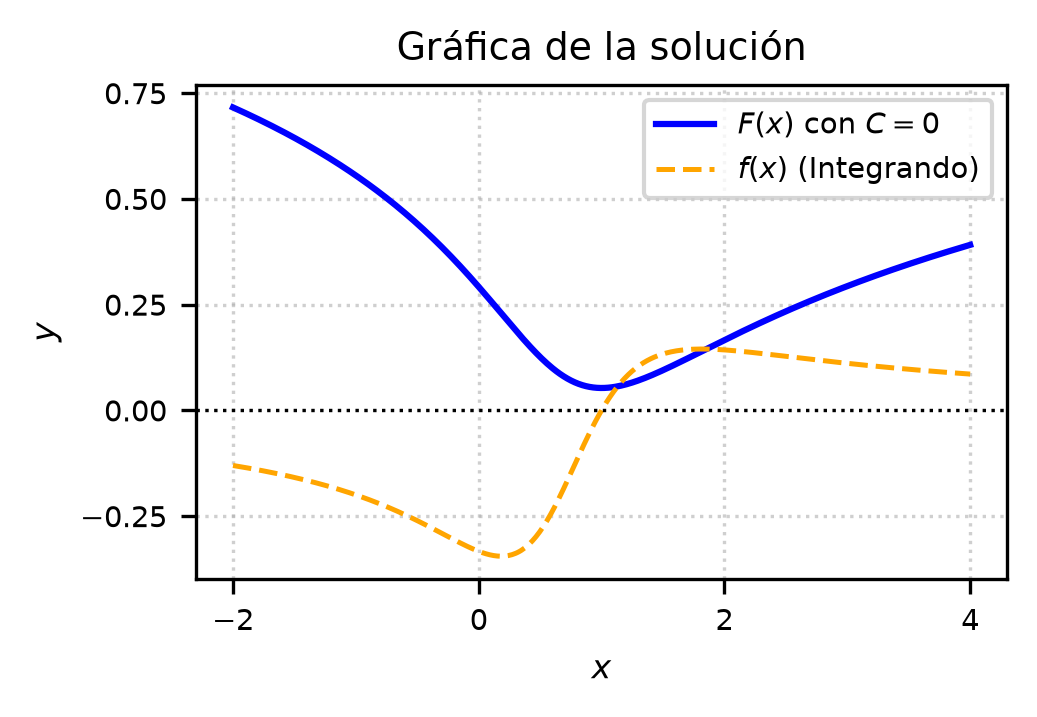
\includegraphics[width=\columnwidth]{semana_03/graficas/SEM03_P02_grafica.png}
	\caption{Representación gráfica de $f(x)$ y su antiderivada $F(x)$ evaluada para la constante de integración $C = 0$ (Problema 02).}
	\label{fig:problema02}
\end{figure}
